%%%%%%%%%%%%%%%%%%%%%%%%%%%%%%%%%%%%%%%%%%%%%%%%%%%%%%%%%%%%%%%%%%%%%%%%%%%%%%%%%%%%%%%%%%%%%%%%%%%%%%
% Plantilla básica de Latex en Español.
%
% Autor: Andrés Herrera Poyatos (https://github.com/andreshp)
%
% Es una plantilla básica para redactar documentos. Utiliza el paquete fancyhdr para darle un
% estilo moderno pero serio.
%
% La plantilla se encuentra adaptada al español.
%
%%%%%%%%%%%%%%%%%%%%%%%%%%%%%%%%%%%%%%%%%%%%%%%%%%%%%%%%%%%%%%%%%%%%%%%%%%%%%%%%%%%%%%%%%%%%%%%%%%%%%%

%-----------------------------------------------------------------------------------------------------
%	INCLUSIÓN DE PAQUETES BÁSICOS
%-----------------------------------------------------------------------------------------------------

\documentclass{article}

\usepackage{lipsum}                     % Texto dummy. Quitar en el documento final.

%-----------------------------------------------------------------------------------------------------
%	SELECCIÓN DEL LENGUAJE
%-----------------------------------------------------------------------------------------------------

% Paquetes para adaptar Látex al Español:
\usepackage[spanish,es-noquoting, es-tabla, es-lcroman]{babel} % Cambia
\usepackage[utf8]{inputenc}                                    % Permite los acentos.
\selectlanguage{spanish}                                       % Selecciono como lenguaje el Español.

%-----------------------------------------------------------------------------------------------------
%	SELECCIÓN DE LA FUENTE
%-----------------------------------------------------------------------------------------------------

% Fuente utilizada.
\usepackage{courier}                    % Fuente Courier.
\usepackage{microtype}                  % Mejora la letra final de cara al lector.

%-----------------------------------------------------------------------------------------------------
%	ESTILO DE PÁGINA
%-----------------------------------------------------------------------------------------------------

% Paquetes para el diseño de página:
\usepackage{fancyhdr}               % Utilizado para hacer títulos propios.
\usepackage{lastpage}               % Referencia a la última página. Utilizado para el pie de página.
\usepackage{extramarks}             % Marcas extras. Utilizado en pie de página y cabecera.
\usepackage[parfill]{parskip}       % Crea una nueva línea entre párrafos.
\usepackage{geometry}               % Asigna la "geometría" de las páginas.

% Se elige el estilo fancy y márgenes de 3 centímetros.
\pagestyle{fancy}
\geometry{left=3cm,right=3cm,top=3cm,bottom=3cm,headheight=1cm,headsep=0.5cm} % Márgenes y cabecera.
% Se limpia la cabecera y el pie de página para poder rehacerlos luego.
\fancyhf{}

% Espacios en el documento:
\linespread{1.1}                        % Espacio entre líneas.
\setlength\parindent{0pt}               % Selecciona la indentación para cada inicio de párrafo.
\usepackage{hyperref}
% Cabecera del documento. Se ajusta la línea de la cabecera.
\renewcommand\headrule{
	\begin{minipage}{1\textwidth}
	    \hrule width \hsize
	\end{minipage}
}

% Texto de la cabecera:
\lhead{\docauthor}                          % Parte izquierda.
\chead{}                                    % Centro.
\rhead{\subject \ - \doctitle}              % Parte derecha.

% Pie de página del documento. Se ajusta la línea del pie de página.
\renewcommand\footrule{
\begin{minipage}{1\textwidth}
    \hrule width \hsize
\end{minipage}\par
}

\lfoot{}                                                 % Parte izquierda.
\cfoot{}                                                 % Centro.
\rfoot{Página\ \thepage\ de\ \protect\pageref{LastPage}} % Parte derecha.


%-----------------------------------------------------------------------------------------------------
%	PORTADA
%-----------------------------------------------------------------------------------------------------

% Elija uno de los siguientes formatos.
% No olvide incluir los archivos .sty asociados en el directorio del documento.
\usepackage{title1}
%\usepackage{title2}

%-----------------------------------------------------------------------------------------------------
%	TÍTULO, AUTOR Y OTROS DATOS DEL DOCUMENTO
%-----------------------------------------------------------------------------------------------------

% Título del documento.
\newcommand{\doctitle}{Algoritmos genéticos y Differential Evolution en Sentiment Analysis}
% Subtítulo.
 \newcommand{\docsubtitle}{}
% Fecha.
\newcommand{\docdate}{1 \ de \ Enero \ de \ 2015}
% Asignatura.
\newcommand{\subject}{Metaheurísticas}
% Autor.
\newcommand{\docauthor}{Nuria Rodríguez Barroso}
\newcommand{\docaddress}{Universidad de Granada}
\newcommand{\docemail}{rbnuria@correo.ugr.es}

%-----------------------------------------------------------------------------------------------------
%	RESUMEN
%-----------------------------------------------------------------------------------------------------

% Resumen del documento. Va en la portada.
% Puedes también dejarlo vacío, en cuyo caso no aparece en la portada.
%\newcommand{\docabstract}{}
\newcommand{\docabstract}{Aplicación de algoritmos genéticos y Differential evolution para la optimización del comportamiento de herramientas de extracción de polaridad}

\begin{document}

\maketitle

%-----------------------------------------------------------------------------------------------------
%	ÍNDICE
%-----------------------------------------------------------------------------------------------------

% Profundidad del Índice:
%\setcounter{tocdepth}{1}

\newpage
\tableofcontents
\newpage

%-----------------------------------------------------------------------------------------------------
%	SECCIÓN 1
%-----------------------------------------------------------------------------------------------------

\section{Introducción}

	\subsection{Contexto}
	En los últimos años, la minería de datos ha obtenido tal relevancia en nuestra sociedad que cada vez se considera más indispensable a la hora de la toma de decisiones en una corporación. Estamos rodeados de todo tipo de datos: afinidades, ubicaciones, opiniones, información personal, etc.
	
	Una corporación o empresa, como sabemos, ofrece un producto al cliente con el fin de satisfacerlo y además lucrarse. Sería de gran interés para esta empresa conocer cuál es la opinión del cliente sobre el producto, cuáles son las mejoras que él añadiría y cuáles son los defectos que él eliminaría. 
	
	Actualmente, obtener una opinión de un cliente sobre tu producto es mucho más fácil que pasar una encuesta, gracias a la Web 2.0. Basta con analizar las redes sociales, que están en continuo crecimiento, o analizar otras fuentes de opiniones como pueden ser TripAdvisor, Google, Amazon,etc. Pero, ¿cómo analizaríamos estas opiniones, sobre todo cuando tu producto es comprado y valorado por miles de personas? Efectivamente, hacerlo contratando personal que valore estos comentarios resultaría inviable, tanto por el tiempo que llevaría como por los recursos económicos que habría que invertir.
	
	Sentiment Analysis pretende dar una solución a este problema.  Se trata de un campo de la minería de datos que, según \cite{tanetal}, se centra en la extracción de información útil a partir de textos. Este tema cada vez está obteniendo mayor popularidad en el ámbito de la computación. Como vemos en la figura \ref{fig:relevancia} obtenida a partir de Google Trends, durante los últimos años, Sentiment Analysis ha ido ganado popularidad en las búsquedas, un claro reflejo de que se trata de un campo cada vez más importante y útil.
\begin{figure}[h]
	\centering
	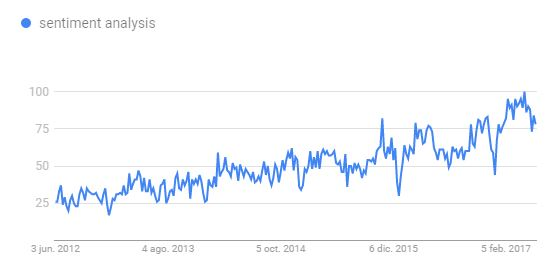
\includegraphics[width=0.7\linewidth]{relevancia}
	\caption{Relevancia del Sentiment Analysis según las búsquedas realizadas en Google}
	\label{fig:relevancia}
\end{figure}
\newpage
\subsection{Sentiment Analysis y descripción del problema}
Sentiment Analysis podría definirse como un problema de clasificación (ver \ref{fig:clasificationscheme}) en el que el objetivo es identificar el sentimiento que un texto transmite. Se trata de un problema cuya principal dificultad recae en el tratamiento de información difusa, en la que además de factores más objetivos como la ortografía, existen también otros factores subjetivos tales como la ironía o el sarcasmo, a veces siendo estos difíciles de entender incluso por los seres humanos.

Para obtener esta clasificación, existen varias alternativas:
\begin{itemize}
	\item \textbf{Aproximación por Aprendizaje Automático.} El problema se trata con técnicas de aprendizaje automático tales como Support Vector Machine o técnicas basadas en árboles. Pueden ser problemas supervisados o no supervisados. En los primeros el principal problema es que debemos tener un gran conjunto de comentarios ya etiquetados con el fin de aprender a partir de estos comentarios etiquetados. En los segundos, nuestro sentimiento se extrae a partir de funciones heurísticas u otras reglas predefinida.
	\item \textbf{Aproximación por técnicas basadas en diccionarios.} Estas técnicas se basan en diccionarios elaborados manualmente donde cada palabra tiene una intensidad de sentimiento asociada. Alternativamente a las técnicas basadas en diccionarios tenemos las técnicas basadas en corpus, donde se tienen en cuenta distintos patrones sintácticos tales como palabras que expresan conectividad o por ejemplo contradicción.
	\item  \textbf{Aproximación por herramientas de Procesamiento del Lenguaje Natural (NLP).} Estas herramientas emplean técnicas computacionales (Aprendizaje automático, inteligenia artificial, inferencia estadística...) unidas a técnicas basadas en lingüística para darnos la polaridad de un texto. Se puede definir también como un software que integra alguna de las 2 técnicas nombradas anteriormente (o ambas) y que ha sido desarrollado con fines comerciales o de investigación, facilitando al usuario el proceso de Sentiment Analysis (sin que este tenga que desarrollar su propio modelo o su propio diccionario).
\end{itemize}

\begin{figure}
	\centering
	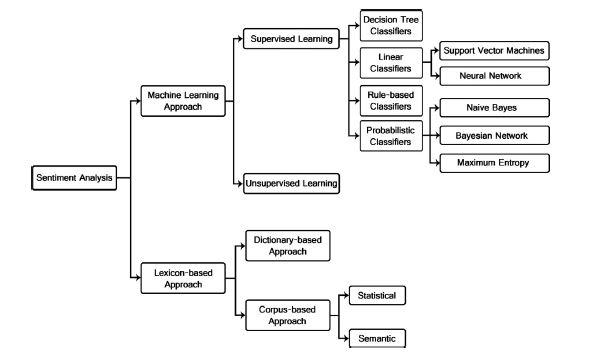
\includegraphics[width=0.7\linewidth]{clasificationScheme}
	\caption{Esquema del problema de Sentiment Analysis}
	\label{fig:clasificationscheme}
\end{figure}

\newpage
\textbf{Nuestro problema}

Nuestro problema consiste en la optimización del comportamiento de 7 herramientas de Procesamiento de Lenguaje Natural (NLP) o herramientas de extracción de polaridad con respecto al etiquetado experto de un total de 20 datasets de comentarios y la comparación de los resultados con otras alternativas tales como la agregación de estas herramientas (entre otras). Esta optimización del comportamiento se realizará mediante la asignación de pesos a las herramientas, siendo estos pesos buscados mediante algoritmos genéticos primero y posteriormente técnicas de Differential Evolution.

Partiremos de las intensidades que cada herramienta nos devuelve para cada comentario y nuestro objetivo es que la combinación lineal de las intensidades de cada herramienta ponderadas con el peso de la solución minimice primero el error de clasificación (primeros experimentos) y el posterior error cuadrático.
%-----------------------------------------------------------------------------------------------------
%	SECCIÓN 2
%-----------------------------------------------------------------------------------------------------}
\begin{thebibliography}{99}
\bibitem[Tan et al., 1999]{tanetal} \hspace{-.22cm} Tan, A.-H. et al. (1999), Text mining: The state of the art and
	the challenges. In Proceedings of the PAKDD 1999 Workshop on Knowledge
	Disocovery from Advanced Databases, volume 8, pages 65-70.
\end{thebibliography}
\end{document}
